\documentclass[12pt,a4paper]{article}
\usepackage[margin=1in]{geometry}
\usepackage{graphicx}
\usepackage{amsmath}
\usepackage{hyperref}
\usepackage{enumitem}
\usepackage{float}
\usepackage{booktabs}
\usepackage{caption}
\usepackage{subcaption}
\usepackage{authblk}
\usepackage[backend=biber]{biblatex}
\addbibresource{references.bib}

\title{Achieving 94\% Accuracy on CIFAR-10: A Deep Learning Approach}
\author{Jan Stratmann \\ TU Dortmund University}
\date{\today}

\begin{document}
\maketitle

\section{Introduction}
The CIFAR-10 dataset is a widely used benchmark in the field of computer vision, consisting of 60,000 color images in 10 distinct classes\cite{krizhevsky2009}. Each image is of size $32 \times 32$ pixels, and the dataset is split into 50,000 training images and 10,000 test images. The goal of this project is to develop a convolutional neural network (CNN) to achieve at least 90\% accuracy on this dataset. Through the use of data augmentation, learning rate scheduling, and careful model design, the final model achieves 94\% accuracy, demonstrating the effectiveness of modern deep learning techniques for image classification tasks.

\section{Dataset and Preprocessing}
The CIFAR-10 dataset contains small, low-resolution images representing a variety of objects such as airplanes, automobiles, birds, and cats. Due to the limited size and resolution, effective preprocessing and augmentation are crucial for achieving high accuracy. In this project, several data augmentation techniques are applied to the training images to improve generalization and prevent overfitting. Color jitter is used to randomly change the brightness, contrast, saturation, and hue of the images. Perspective transforms are applied to simulate different viewpoints, and random horizontal flips are performed with a 50\% probability. These augmentations help the model learn more robust features and improve its performance on unseen data.

\section{Model Architecture}
The neural network used in this project is inspired by the AlexNet architecture\cite{krizhevsky2012imagenet}, but adapted for the smaller input size of CIFAR-10 images. The model consists of multiple convolutional layers with increasing channel sizes, interleaved with batch normalization and ReLU activation functions. Max pooling layers are used to reduce the spatial dimensions, and dropout is applied for regularization. The feature extractor is followed by fully connected layers that perform the final classification into the 10 CIFAR-10 classes.

The architecture can be summarized as follows:
\begin{itemize}
    \item \textbf{Feature extractor:}
        \begin{itemize}
            \item Block 1: Conv2d (3$\rightarrow$64), BatchNorm2d, ReLU; Conv2d (64$\rightarrow$128), ReLU; Conv2d (128$\rightarrow$128), ReLU; MaxPool2d.
            \item Block 2: Conv2d (128$\rightarrow$256), BatchNorm2d, ReLU; two Conv2d (256$\rightarrow$256), each with ReLU; MaxPool2d; Dropout (0.2).
            \item Block 3: Conv2d (256$\rightarrow$512), BatchNorm2d, ReLU; two Conv2d (512$\rightarrow$512), each with ReLU; MaxPool2d; Dropout (0.2).
    \end{itemize}
    \item \textbf{Classifier:}
    \begin{itemize}
        \item Flatten the output of the feature extractor.
        \item Linear layer (flattened dimension$\rightarrow$1024), ReLU.
        \item Linear layer (1024$\rightarrow$256), ReLU, Dropout (0.2).
        \item Linear layer (256$\rightarrow$10) for final class prediction.
    \end{itemize}
\end{itemize}
This architecture uses batch normalization, dropout, and ReLU activations throughout, and is specifically adapted for the $32\times32$ CIFAR-10 images.

\section{Training Setup}
The model is implemented in PyTorch and trained using stochastic gradient descent (SGD) with a learning rate of 0.01, momentum of 0.9, and weight decay of $5 \times 10^{-4}$. Cross-entropy loss is used as the objective function, which is suitable for multi-class classification tasks. Training is performed with a batch size of 128 images over 100 epochs on an NVIDIA GTX 3060 GPU with 12GB VRAM. MLflow is utilized for experiment tracking, logging training metrics and model checkpoints, while FiftyOne is employed for in-depth analysis and visualization of model predictions. Additionally, cosine learning rate scheduling is applied to further improve performance by reducing the learning rate during training.

\section{Results}
The effectiveness of the proposed approach is demonstrated through a series of experiments:
\begin{itemize}
    \item \textbf{Vanilla training:} Without data augmentation or learning rate scheduling, the model achieves 88.3\% accuracy.
    \item \textbf{With data augmentation:} Incorporating augmentation techniques increases accuracy to 92.5\%.
    \item \textbf{With learning rate scheduling:} Further improvements with learning rate scheduling result in a final accuracy of 94\%.
\end{itemize}
These results highlight the importance of both data augmentation and learning rate scheduling in achieving state-of-the-art performance on CIFAR-10 with a relatively simple CNN architecture.
\begin{figure}[H]
    \centering
    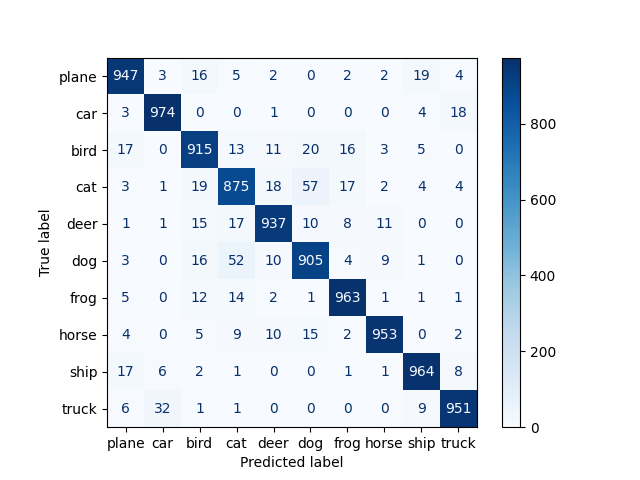
\includegraphics[width=0.6\textwidth]{figures/confusion_matrix.png}
    \caption{Confusion matrix of the final model on the CIFAR-10 test set, demonstrating high accuracy across all classes.}
    \label{fig:confusion_matrix}
\end{figure}
The confusion matrix in Figure \ref{fig:confusion_matrix} illustrates the model's performance across all classes, showing that it effectively distinguishes between different categories with minimal misclassifications. The most common misclassifications occur between visually similar classes, such as cats and dogs.

The source code for the model and training pipeline is available at \url{https://github.com/jstr01/cifar10-classifier}.

\section{Conclusion}
This project demonstrates that with careful model design, data augmentation, and training strategies, it is possible to achieve high accuracy on the CIFAR-10 dataset using a relatively simple CNN architecture. The use of MLflow and FiftyOne further enhances the experiment tracking and analysis process, making it easier to iterate and improve upon the model. The techniques presented here can serve as a strong baseline for future work on small image classification tasks.

\section*{References}
\printbibliography[heading=none]

\end{document}
